\documentclass[a4paper]{article}

\def\npart {IB}
\def\nterm {Lent}
\def\nyear {2016}
\def\nlecturer {A. G. Kovalev}
\def\ncourse {Geometry}
\def\nlectures {TT.10}
\def\nnotready {}

% Imports
\ifx \nextra \undefined
  \usepackage[pdftex,
    hidelinks,
    pdfauthor={Dexter Chua},
    pdfsubject={Cambridge Maths Notes: Part \npart\ - \ncourse},
    pdftitle={Part \npart\ - \ncourse},
  pdfkeywords={Cambridge Mathematics Maths Math \npart\ \nterm\ \nyear\ \ncourse}]{hyperref}
  \title{Part \npart\ - \ncourse}
\else
  \usepackage[pdftex,
    hidelinks,
    pdfauthor={Dexter Chua},
    pdfsubject={Cambridge Maths Notes: Part \npart\ - \ncourse\ (\nextra)},
    pdftitle={Part \npart\ - \ncourse\ (\nextra)},
  pdfkeywords={Cambridge Mathematics Maths Math \npart\ \nterm\ \nyear\ \ncourse\ \nextra}]{hyperref}

  \title{Part \npart\ - \ncourse \\ {\Large \nextra}}
\fi

\author{Lectured by \nlecturer \\\small Notes taken by Dexter Chua}
\date{\nterm\ \nyear}

\usepackage{alltt}
\usepackage{amsfonts}
\usepackage{amsmath}
\usepackage{amssymb}
\usepackage{amsthm}
\usepackage{booktabs}
\usepackage{caption}
\usepackage{enumitem}
\usepackage{fancyhdr}
\usepackage{graphicx}
\usepackage{mathtools}
\usepackage{microtype}
\usepackage{multirow}
\usepackage{pdflscape}
\usepackage{pgfplots}
\usepackage{siunitx}
\usepackage{tabularx}
\usepackage{tikz}
\usepackage{tkz-euclide}
\usepackage[normalem]{ulem}
\usepackage[all]{xy}

\pgfplotsset{compat=1.12}

\pagestyle{fancyplain}
\lhead{\emph{\nouppercase{\leftmark}}}
\ifx \nextra \undefined
  \rhead{
    \ifnum\thepage=1
    \else
      \npart\ \ncourse
    \fi}
\else
  \rhead{
    \ifnum\thepage=1
    \else
      \npart\ \ncourse\ (\nextra)
    \fi}
\fi
\usetikzlibrary{arrows}
\usetikzlibrary{decorations.markings}
\usetikzlibrary{decorations.pathmorphing}
\usetikzlibrary{positioning}
\usetikzlibrary{fadings}
\usetikzlibrary{intersections}
\usetikzlibrary{cd}

\newcommand*{\Cdot}{\raisebox{-0.25ex}{\scalebox{1.5}{$\cdot$}}}
\newcommand {\pd}[2][ ]{
  \ifx #1 { }
    \frac{\partial}{\partial #2}
  \else
    \frac{\partial^{#1}}{\partial #2^{#1}}
  \fi
}

% Theorems
\theoremstyle{definition}
\newtheorem*{aim}{Aim}
\newtheorem*{axiom}{Axiom}
\newtheorem*{claim}{Claim}
\newtheorem*{cor}{Corollary}
\newtheorem*{defi}{Definition}
\newtheorem*{eg}{Example}
\newtheorem*{fact}{Fact}
\newtheorem*{law}{Law}
\newtheorem*{lemma}{Lemma}
\newtheorem*{notation}{Notation}
\newtheorem*{prop}{Proposition}
\newtheorem*{thm}{Theorem}

\renewcommand{\labelitemi}{--}
\renewcommand{\labelitemii}{$\circ$}
\renewcommand{\labelenumi}{(\roman{*})}

\let\stdsection\section
\renewcommand\section{\newpage\stdsection}

% Strike through
\def\st{\bgroup \ULdepth=-.55ex \ULset}

% Maths symbols
\newcommand{\bra}{\langle}
\newcommand{\ket}{\rangle}

\newcommand{\N}{\mathbb{N}}
\newcommand{\Z}{\mathbb{Z}}
\newcommand{\Q}{\mathbb{Q}}
\renewcommand{\H}{\mathbb{H}}
\newcommand{\R}{\mathbb{R}}
\newcommand{\C}{\mathbb{C}}
\newcommand{\Prob}{\mathbb{P}}
\renewcommand{\P}{\mathbb{P}}
\newcommand{\E}{\mathbb{E}}
\newcommand{\F}{\mathbb{F}}
\newcommand{\cU}{\mathcal{U}}
\newcommand{\RP}{\mathbb{RP}}
\newcommand{\CP}{\mathbb{CP}}

\newcommand{\ph}{\,\cdot\,}

\DeclareMathOperator{\sech}{sech}
\DeclareMathOperator{\cosech}{cosech}
\DeclareMathOperator{\cosec}{cosec}

\DeclareMathOperator{\covol}{covol}
\DeclareMathOperator{\vol}{vol}

\let\Im\relax
\let\Re\relax
\DeclareMathOperator{\Im}{Im}
\DeclareMathOperator{\Re}{Re}
\DeclareMathOperator{\im}{im}
\DeclareMathOperator{\image}{image}
\DeclareMathOperator{\Ann}{Ann}

\DeclareMathOperator*{\res}{res}
\DeclareMathOperator{\Res}{Res}
\DeclareMathOperator{\Ind}{Ind}

\DeclareMathOperator{\tr}{tr}
\DeclareMathOperator{\diag}{diag}
\DeclareMathOperator{\rank}{rank}
\DeclareMathOperator{\card}{card}
\DeclareMathOperator{\spn}{span}
\DeclareMathOperator{\adj}{adj}

\DeclareMathOperator{\erf}{erf}
\DeclareMathOperator{\erfc}{erfc}

\DeclareMathOperator{\ord}{ord}
\DeclareMathOperator{\Sym}{Sym}

\DeclareMathOperator{\sgn}{sgn}
\DeclareMathOperator{\orb}{orb}
\DeclareMathOperator{\stab}{stab}
\DeclareMathOperator{\ccl}{ccl}

\DeclareMathOperator{\lcm}{lcm}
\DeclareMathOperator{\hcf}{hcf}

\DeclareMathOperator{\Int}{Int}
\DeclareMathOperator{\id}{id}

\DeclareMathOperator{\betaD}{beta}
\DeclareMathOperator{\gammaD}{gamma}
\DeclareMathOperator{\Poisson}{Poisson}
\DeclareMathOperator{\binomial}{binomial}
\DeclareMathOperator{\multinomial}{multinomial}
\DeclareMathOperator{\Bernoulli}{Bernoulli}
\DeclareMathOperator{\like}{like}

\DeclareMathOperator{\var}{var}
\DeclareMathOperator{\cov}{cov}
\DeclareMathOperator{\bias}{bias}
\DeclareMathOperator{\mse}{mse}
\DeclareMathOperator{\corr}{corr}

\DeclareMathOperator{\otp}{otp}
\DeclareMathOperator{\dom}{dom}

\DeclareMathOperator{\Root}{Root}
\DeclareMathOperator{\supp}{supp}
\DeclareMathOperator{\rel}{rel}
\DeclareMathOperator{\Hom}{Hom}
\DeclareMathOperator{\Aut}{Aut}
\DeclareMathOperator{\Gal}{Gal}
\DeclareMathOperator{\Mat}{Mat}
\DeclareMathOperator{\End}{End}
\DeclareMathOperator{\Char}{char}
\DeclareMathOperator{\ev}{ev}
\DeclareMathOperator{\St}{St}
\DeclareMathOperator{\Lk}{Lk}
\DeclareMathOperator{\disc}{disc}
\DeclareMathOperator{\Isom}{Isom}
\DeclareMathOperator{\length}{length}
\DeclareMathOperator{\energy}{energy}
\DeclareMathOperator{\area}{area}
\DeclareMathOperator{\Syl}{Syl}
\DeclareMathOperator{\cl}{cl}
\DeclareMathOperator{\fix}{fix}

\newcommand{\GL}{\mathrm{GL}}
\newcommand{\SL}{\mathrm{SL}}
\newcommand{\PGL}{\mathrm{PGL}}
\newcommand{\PSL}{\mathrm{PSL}}
\newcommand{\PSU}{\mathrm{PSU}}
\newcommand{\Or}{\mathrm{O}}
\newcommand{\SO}{\mathrm{SO}}
\newcommand{\U}{\mathrm{U}}
\newcommand{\SU}{\mathrm{SU}}

\renewcommand{\d}{\mathrm{d}}
\newcommand{\D}{\mathrm{D}}

\tikzset{->/.style = {decoration={markings,
                                  mark=at position 1 with {\arrow[scale=2]{latex'}}},
                      postaction={decorate}}}
\tikzset{<-/.style = {decoration={markings,
                                  mark=at position 0 with {\arrowreversed[scale=2]{latex'}}},
                      postaction={decorate}}}
\tikzset{<->/.style = {decoration={markings,
                                   mark=at position 0 with {\arrowreversed[scale=2]{latex'}},
                                   mark=at position 1 with {\arrow[scale=2]{latex'}}},
                       postaction={decorate}}}
\tikzset{->-/.style = {decoration={markings,
                                   mark=at position #1 with {\arrow[scale=2]{latex'}}},
                       postaction={decorate}}}
\tikzset{-<-/.style = {decoration={markings,
                                   mark=at position #1 with {\arrowreversed[scale=2]{latex'}}},
                       postaction={decorate}}}

\tikzset{circ/.style = {fill, circle, inner sep = 0, minimum size = 3}}
\tikzset{mstate/.style={circle, draw, blue, text=black, minimum width=0.7cm}}

\definecolor{mblue}{rgb}{0.2, 0.3, 0.8}
\definecolor{morange}{rgb}{1, 0.5, 0}
\definecolor{mgreen}{rgb}{0.1, 0.4, 0.2}
\definecolor{mred}{rgb}{0.5, 0, 0}

\def\drawcirculararc(#1,#2)(#3,#4)(#5,#6){%
    \pgfmathsetmacro\cA{(#1*#1+#2*#2-#3*#3-#4*#4)/2}%
    \pgfmathsetmacro\cB{(#1*#1+#2*#2-#5*#5-#6*#6)/2}%
    \pgfmathsetmacro\cy{(\cB*(#1-#3)-\cA*(#1-#5))/%
                        ((#2-#6)*(#1-#3)-(#2-#4)*(#1-#5))}%
    \pgfmathsetmacro\cx{(\cA-\cy*(#2-#4))/(#1-#3)}%
    \pgfmathsetmacro\cr{sqrt((#1-\cx)*(#1-\cx)+(#2-\cy)*(#2-\cy))}%
    \pgfmathsetmacro\cA{atan2(#2-\cy,#1-\cx)}%
    \pgfmathsetmacro\cB{atan2(#6-\cy,#5-\cx)}%
    \pgfmathparse{\cB<\cA}%
    \ifnum\pgfmathresult=1
        \pgfmathsetmacro\cB{\cB+360}%
    \fi
    \draw (#1,#2) arc (\cA:\cB:\cr);%
}
\newcommand\getCoord[3]{\newdimen{#1}\newdimen{#2}\pgfextractx{#1}{\pgfpointanchor{#3}{center}}\pgfextracty{#2}{\pgfpointanchor{#3}{center}}}

\def\Xint#1{\mathchoice
   {\XXint\displaystyle\textstyle{#1}}%
   {\XXint\textstyle\scriptstyle{#1}}%
   {\XXint\scriptstyle\scriptscriptstyle{#1}}%
   {\XXint\scriptscriptstyle\scriptscriptstyle{#1}}%
   \!\int}
\def\XXint#1#2#3{{\setbox0=\hbox{$#1{#2#3}{\int}$}
     \vcenter{\hbox{$#2#3$}}\kern-.5\wd0}}
\def\ddashint{\Xint=}
\def\dashint{\Xint-}


\begin{document}
\maketitle
{\small
\noindent Groups of rigid motions of Euclidean space. Rotation and reflection groups in two and three dimensions. Lengths of curves.\hspace*{\fill} [2]

\vspace{5pt}
\noindent Spherical geometry: spherical lines, spherical triangles and the Gauss-Bonnet theorem. Stereographic projection and M\"obius transformations.\hspace*{\fill} [3]

\vspace{5pt}
\noindent Triangulations of the sphere and the torus, Euler number.\hspace*{\fill} [1]

\vspace{5pt}
\noindent Riemannian metrics on open subsets of the plane. The hyperbolic plane. Poincar\'e models and their metrics. The isometry group. Hyperbolic triangles and the Gauss-Bonnet theorem. The hyperboloid model.\hspace*{\fill} [4]

\vspace{5pt}
\noindent Embedded surfaces in $\R^3$. The first fundamental form. Length and area. Examples.\hspace*{\fill} [1]

\vspace{5pt}
\noindent Length and energy. Geodesics for general Riemannian metrics as stationary points of the energy. First variation of the energy and geodesics as solutions of the corresponding Euler-Lagrange equations. Geodesic polar coordinates (informal proof of existence). Surfaces of revolution.\hspace*{\fill} [2]

\vspace{5pt}
\noindent The second fundamental form and Gaussian curvature. For metrics of the form $du^2 + G(u, v) dv^2$, expression of the curvature as $\sqrt{G_{uu}}/\sqrt{G}$. Abstract smooth surfaces and isometries. Euler numbers and statement of Gauss-Bonnet theorem, examples and applications.\hspace*{\fill} [3]}

\tableofcontents
\section{Euclidean geometry}
\subsection{Isometrics of the Euclidean plane}
We are first going to look at Euclidean geometry. Roughly, this is the geometry of $\R^n$ under the usual inner product and norm.

\begin{defi}[(Standard) inner product]
  The \emph{(standard) inner product} on $\R^n$ is defined by
  \[
    (\mathbf{x}, \mathbf{y}) = \mathbf{x}\cdot \mathbf{y} = \sum_{i = 1}^n x_i y_i.
  \]
\end{defi}

\begin{defi}[Euclidean Norm]
  The \emph{Euclidean norm} of $\mathbf{x} \in \R^n$ is
  \[
    \|\mathbf{x}\| = \sqrt{(\mathbf{x}, \mathbf{x})}.
  \]
  This defines a metric on $\R^n$ by
  \[
    d(\mathbf{x}, \mathbf{y}) = \|\mathbf{x} - \mathbf{y}\|.
  \]
\end{defi}

\begin{defi}[Isometry]
  A map $f: \R^n \to \R^n$ is an \emph{isometry} of $\R^n$ if
  \[
    d(f(\mathbf{x}), f(\mathbf{y})) = d(\mathbf{x}, \mathbf{y})
  \]
  for all $\mathbf{x}, \mathbf{y} \in \R^n$.
\end{defi}
Note that $f$ is not required to be linear.

We would like to see some examples of isometries. A good source of examples is matrices. Recall the following definition:
\begin{defi}[Orthogonal matrix]
  An $n \times n$ matrix $A$ is \emph{orthogonal} if $AA^T = A^T A = I$. The group of all orthogonal matrices is the orthogonal group $\Or(n)$.
\end{defi}

In general, for any matrix $A$ and $\mathbf{x}, \mathbf{y} \in \R^n$, we get
\[
  (A\mathbf{x}, A \mathbf{y}) = (A\mathbf{x})^T (A \mathbf{y}) = \mathbf{x}^T A^T A \mathbf{y} = (\mathbf{x}, A^T A \mathbf{y}).
\]
So $A$ is orthogonal if and only if $(A\mathbf{x}, A\mathbf{y}) = (\mathbf{x}, \mathbf{y})$ for all $\mathbf{x}, \mathbf{y} \in \R^n$.

Recall also that the inner product can be expressed in terms of the norm by
\[
  (\mathbf{x}, \mathbf{y}) = \frac{1}{2}(\|\mathbf{x} + \mathbf{y}\|^2 - \|\mathbf{x}\|^2 -\|\mathbf{y}\|^2).
\]
So if $A$ preserves in norm, then it preserves the inner product, and the converse is obviously true. So $A$ is orthogonal if and only if $\|A\mathbf{x}\| = \|\mathbf{x}\|$ for all $\mathbf{x} \in \R^n$. Hence matrices are orthogonal if and only if they are isometries.

More generally, let
\[
  f(\mathbf{x}) = A\mathbf{x} + \mathbf{b}.
\]
Then
\[
  d(f(\mathbf{x}), f(\mathbf{y})) = \|A(\mathbf{x} - \mathbf{y})\|.
\]
So any $f$ of this form is an isometry if and only if $A$ is orthogonal. This is not too surprising. What might not be expected is that all isometries are of this form.

\begin{thm}
  Every isometry of $f: \R^n \to \R^n$ is of the form
  \[
    f(\mathbf{x}) = A\mathbf{x} + \mathbf{b}.
  \]
  for $A$ orthogonal and $\mathbf{b} \in \R^n$.
\end{thm}

\begin{proof}
  Let $f$ be an isometry. Let $\mathbf{e}_1, \cdots, \mathbf{e}_n$ be the standard basis of $\R^n$. Let
  \[
    \mathbf{b} = f(\mathbf{0}), \quad \mathbf{a}_i = f(\mathbf{e}_i) - \mathbf{b}.
  \]
  The idea is to construct our matrix $A$ out of these $\mathbf{a}_i$. For $A$ to be orthogonal, $\{\mathbf{a}_i\}$ must be an orthonormal basis.

  Indeed, we can compute
  \[
    \|\mathbf{a}_i\| = \|\mathbf{f}(\mathbf{e}_i) - f(\mathbf{0})\| = d(f(\mathbf{e}_i), f(\mathbf{0})) = d(\mathbf{e}_i, \mathbf{0}) = \|\mathbf{e}_i\| = 1.
  \]
  For $i \not = j$, we have
  \begin{align*}
    (\mathbf{a}_i, \mathbf{a}_j) &= -(\mathbf{a}_i, -\mathbf{a}_j) \\
    &=-\frac{1}{2}(\|\mathbf{a}_i - \mathbf{a}_j\|^2 - \|\mathbf{a}_i\|^2 - \mathbf{a}_j\|^2)\\
    &= -\frac{1}{2}(\|f(\mathbf{e}_i) - f(\mathbf{e}_j)\|^2 - 2)\\
    &= -\frac{1}{2}(\|\mathbf{e}_i - \mathbf{e}_j\|^2 - 2)\\
    &= 0
  \end{align*}
  So $\mathbf{a}_i$ and $\mathbf{a}_j$ are orthogonal. In other words, $\{\mathbf{a}_i\}$ forms an orthonormal set. It is an easy result that any orthogonal set must be linearly independent. Since we have found $n$ orthonormal vectors, they form an orthonormal basis.

  Hence, the matrix $A$ with columns given by the column vectors $\mathbf{a}_i$ is an orthogonal matrix. We define a new isometry
  \[
    g(\mathbf{x}) = A\mathbf{x} + \mathbf{b}.
  \]
  We want to show $f = g$. By construction, we know $g(\mathbf{x}) = f(\mathbf{x})$ is true for $\mathbf{x} = \mathbf{0}, \mathbf{e}_1, \cdots, \mathbf{e}_n$.

  We observe that $g$ is invertible. In particular,
  \[
    g^{-1}(\mathbf{x}) = A^{-1}(\mathbf{x} - \mathbf{b}) = A^T \mathbf{x} - A^T\mathbf{b}.
  \]
  Moreover, it is an isometry.

  We define
  \[
    h = g^{-1}\circ f.
  \]
  Since it is a composition of isometries, it is also an isometry. Moreover, it fixes $\mathbf{x} = \mathbf{0}, \mathbf{e}_1, \cdots, \mathbf{e}_n$.

  It currently suffices to prove that $h$ is the identity.

  Let $\mathbf{x} \in \R^n$, and expand it in the basis as
  \[
    \mathbf{x} = \sum_{i = 1}^n x_i \mathbf{e}_i.
  \]
  Let
  \[
    \mathbf{y} = h(\mathbf{x}) = \sum_{i = 1}^n y_i \mathbf{e}_i.
  \]
  We can compute
  \begin{align*}
    d(\mathbf{x}, \mathbf{e}_i)^2 &= (\mathbf{x} - \mathbf{e}_i, \mathbf{x} - \mathbf{e}_i) = \|\mathbf{x}\|^2 + 1 - 2 x_i\\
    d(\mathbf{x}, 0)^2 &= \|\mathbf{x}\|^2.
  \end{align*}
  Similarly, we have
  \begin{align*}
    d(\mathbf{y}, \mathbf{e}_i)^2 &= (\mathbf{y} - \mathbf{e}_i, \mathbf{y} - \mathbf{e}_i) = \|\mathbf{y}\|^2 + 1 - 2 y_i\\
    d(\mathbf{y}, 0)^2 &= \|\mathbf{y}\|^2.
  \end{align*}
  Since $h$ is an isometry and fixes $\mathbf{0}, \mathbf{e}_1, \cdots, \mathbf{e}_n$, and by definition $h(\mathbf{x}) = \mathbf{y}$, we must have
  \[
    d(\mathbf{x}, \mathbf{0}) = d(\mathbf{y}, \mathbf{0}), \quad d(\mathbf{x}, \mathbf{e}_i) = d(\mathbf{y}, \mathbf{e}_i).
  \]
  These give $\|\mathbf{x}\|^2 = \|\mathbf{y}\|^2$, and hence $x_i = y_i$ for all $i$. In other words, $\mathbf{x} = \mathbf{y} = h(\mathbf{x})$. So $h$ is the identity.
\end{proof}

\begin{defi}[Isometry group]
  The \emph{isometry group} $\Isom(\R^n)$ is the group of all isometries of $\R^n$, which is a group by composition.
\end{defi}

\begin{eg}[Reflections in an affine hyperplane]
  Let $H \subseteq \R^n$ be an affine hyperplane given by
  \[
    H = \{\mathbf{x} \in \R^n: \mathbf{u} \cdot \mathbf{x} = c\},
  \]
  where $\|\mathbf{u}\| = 1$ and $c \in \R$. This is just a natural generalization of a 2-dimensional plane in $\R^3$. Note that unlike a vector subspace, it does not have to contain the origin.

  Reflection in $H$, written $R_H$, is the map
  \begin{align*}
    R_H: \R^n &\to \R^n\\
    \mathbf{x} &\mapsto \mathbf{x} - 2(\mathbf{x} \cdot \mathbf{u} - c)\mathbf{u}
  \end{align*}
  It is an exercise in the example sheet to show that this is indeed an isometry.

  We now check this is indeed what we think a reflection should be. Note that every point in $\R^n$ can be written as $\mathbf{a} + t\mathbf{u}$, where $\mathbf{a} \in H$. Then the reflection should send this point to $\mathbf{a} - t\mathbf{u}$.
  \begin{center}
    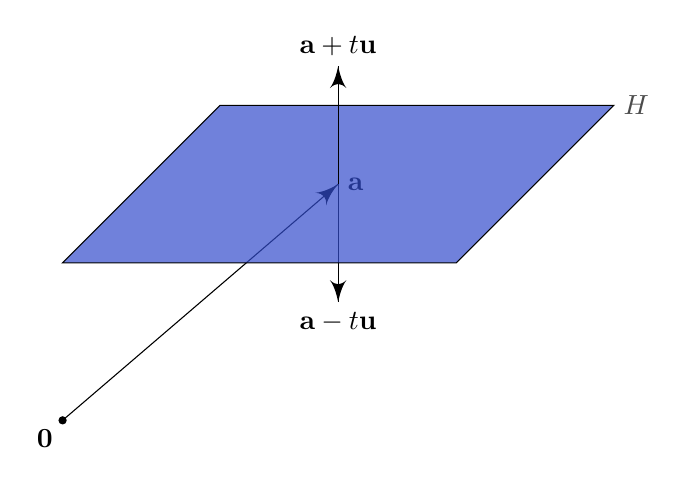
\begin{tikzpicture}
      \node [circ] at (0, -2) {};
      \node [anchor = north east] at (0, -2) {$\mathbf{0}$};
      \draw [->] (0, -2) -- (3.5, 1) node [right] {$\mathbf{a}$};
      \draw [->] (3.5, 1) -- +(0, -1.5) node [below] {$\mathbf{a} - t\mathbf{u}$};
      \draw [fill=mblue, fill opacity=0.7] (0, 0) -- (5, 0) -- (7, 2) node [right] {$H$} -- (2, 2) -- cycle;
      \draw [->] (3.5, 1) -- +(0, 1.5) node [above] {$\mathbf{a} + t\mathbf{u}$};
    \end{tikzpicture}
  \end{center}
  This is a routine check:
  \[
    R_H (\mathbf{a} + t\mathbf{u}) = (\mathbf{a} + t\mathbf{u}) - 2t\mathbf{u} = \mathbf{a} - t\mathbf{u}.
  \]
  In particular, we know $R_H$ fixes exactly the points of $H$.

  The converse is also true --- any isometry $S \in \Isom(\R^n)$ that fixes the points in some affine hyperplane $H$ is either the identity or $R_H$.

  First, we want to translate the plane such that it becomes a vector subspace. Then we can use our linear algebra magic. For any $\mathbf{a} \in \R^n$, we can define the translation by $\mathbf{a}$ as
  \[
    T_{\mathbf{a}}(\mathbf{x}) = \mathbf{x} + \mathbf{a}.
  \]
  This is clearly an isometry.

  We pick an arbitrary $\mathbf{a} \in H$, and let $R = T_{-\mathbf{a}} S T_\mathbf{a} \in \Isom(\R^n)$. Then $R$ fixes exactly $H' = T_{-\mathbf{a}} H$. Since $\mathbf{0} \in H'$, $H'$ is a vector subspace. In particular, if $H = \{\mathbf{x}: \mathbf{x}\cdot \mathbf{u} = c\}$, then by putting $c = \mathbf{a}\cdot \mathbf{u}$, we find
  \[
    H' = \{\mathbf{x}: \mathbf{x}\cdot \mathbf{u} = 0\}.
  \]
  To understand $R$, we already know it fixes everything in $H'$. So we want to see what it does to $\mathbf{u}$. Note that since $R$ is an isometry and fixes the origin, it is in fact an orthogonal map. Hence for any $\mathbf{x} \in H'$, we get
  \[
    (R\mathbf{u}, \mathbf{x}) = (R\mathbf{u}, R\mathbf{x}) = (\mathbf{u}, \mathbf{x}) = 0.
  \]
  So $R\mathbf{u}$ is also perpendicular to $H'$. Hence $R\mathbf{u} = \lambda \mathbf{u}$ for some $\lambda$. Since $R$ is an isometry, we have $\|R\mathbf{u}\|^2 = 1$. Hence $|\lambda|^2 = 1$, and thus $\lambda = \pm 1$. So either $\lambda = 1$, and $R = \id$; or $\lambda = -1$, and $R = R_{H'}$, as we already know for orthogonal matrices.

  It thus follow that $S = \id_{\R^n}$, or $S$ is the reflection in $H$.

  Thus we find that each reflection $R_H$ is the (unique) isometry fixing $H$ but not $\id_{\R^n}$.
\end{eg}
It is an exercise in the example sheet to show that every isometry of $\R^n$ is a composition of at most $n + 1$ reflections. If the isometry fixes $0$, then $n$ reflections will suffice.

Consider the subgroup of $\Isom(\R^n)$ that fixes $\mathbf{0}$. By our general expression for the general isometry, we know this is the set $\{f(\mathbf{x}) = A\mathbf{x}: A A^T = I\} \cong \Or(n)$, the orthogonal group.

For each $A \in \Or(n)$, we must have $\det(A)^2 = 1$. So $\det A = \pm 1$. We use this to define a further subgroup, the special orthogonal group.
\begin{defi}[Special orthogonal group]
  The \emph{special orthogonal gropu} is the group
  \[
    \SO(n) = \{A \in \Or(n):\det A = 1\}.
  \]
\end{defi}

We can look at these explicitly for low dimensions.
\begin{eg}
  Consider
  \[
    A =
    \begin{pmatrix}
      a & b\\
      c & d
    \end{pmatrix} \in \Or(n)
  \]
  Orthogonality then requires
  \[
    a^2 + c^2 = b^2 + d^2 = 1,\quad ab + cd = 0.
  \]
  Now we pick $0 \leq \theta, \varphi \leq 2\pi$ such that
  \begin{align*}
    a &= \cos \theta & b &= -\sin \varphi\\
    c &= \sin \theta & d &= \cos \varphi.
  \end{align*}
  Then $ab + cd = 0$ gives $\tan \theta = \tan \varphi$ (if $\cos \theta$ and $\cos \varphi$ are zero, we formally say these are both infinity). So either $\theta = \varphi$ or $\theta = \varphi \pm \pi$. Thus we have
  \[
    A=
    \begin{pmatrix}
      \cos \theta & -\sin \theta\\
      \sin \theta & \cos \theta
    \end{pmatrix}\text{ or }
    A =
    \begin{pmatrix}
      \cos \theta & \sin \theta\\
      \sin \theta & -\cos \theta
    \end{pmatrix}
  \]
  respectively. In the first case, this is a rotation through $\theta$ about the origin. This is determinant $1$, and hence $A \in \SO(2)$.

  In the second case, this is a reflection in the line $\ell$ at angle $\frac{\theta}{2}$ to the $x$-axis. Then $\det A = -1$ and $A \not\in \SO(2)$.

  So in two dimensions, the orthogonal matrices are either reflections or rotations --- those in $\SO(2)$ are rotations, and the others are reflections.
\end{eg}
Before we can move on to three dimensions, we need to have the notion of orientation. We might intuitively know what an orientation is, but it is rather difficult to define orientation formally. The best we can do is to tell whether two given bases of a vector space have ``the same orientation''. Thus, it would make sense to define an orientation as an equivalence class of bases of ``the same orientation''. We formally define it as follows:
\begin{defi}[Orientation]
  An \emph{orientation} of a vector space is an equivalence class of bases --- let $\mathbf{v}_1, \cdots, \mathbf{v}_n$ and $\mathbf{v}_1', \cdots, \mathbf{v}_n'$ be two bases and $A$ be the change of basis matrix. We say the two bases are equivalent iff $\det A > 0$. This is an equivalence relation on the bases, and the equivalence classes are the orientations.
\end{defi}

\begin{defi}[Orientation-preserving isometry]
  An isometry $f(\mathbf{x}) = A\mathbf{x} + \mathbf{b}$ is \emph{orientation-preserving} if $\det A = 1$. Otherwise, if $\det A = -1$, we say it is \emph{orientation-reversing}.
\end{defi}

\begin{eg}
  We now want to look at $\Or(3)$. First focus on the case where $A \in \SO(3)$, ie. $\det A = 1$. Then we have
  \[
    \det(A - I) = \det(A^T - I) = \det(A)\det(A^T - I) = \det(I - A) = -\det(A - I).
  \]
  So $\det (A - I) = 0$, ie. $+1$ is an eigenvalue in $\R$. So there is some $\mathbf{v}_1 \in \R^3$ such that $A\mathbf{v}_1 = \mathbf{v}_1$.

  We set $W = \bra \mathbf{v}_1\ket^{\perp}$. Let $\mathbf{w} \in W$. Then we can compute
  \[
    (A\mathbf{w}, \mathbf{v}_1) = (A\mathbf{w}, A\mathbf{v}_1) = (\mathbf{w}, \mathbf{v}_1) = 0.
  \]
  So $A\mathbf{w} \in W$. In other words, $W$ is fixed by $A$, and $A|_{W}: W \to W$ is well-defined. Moreover, it is still orthogonal and has determinant $1$. So it is a rotation of the two-dimensional vector space $W$.

  We choose $\{\mathbf{v}_2, \mathbf{v}_3\}$ an orthonormal basis of $W$. Then under the bases $\{\mathbf{v}_1, \mathbf{v}_2, \mathbf{v}_3\}$, $A$ is represented by
  \[
    A =
    \begin{pmatrix}
      1 & 0 & 0\\
      0 & \cos \theta & - \sin \theta\\
      0 & \sin \theta & \cos \theta
    \end{pmatrix}.
  \]
  This is the most general orientation-preserving isometry of $\R^3$ that fixes the origin.

  How about the orientation-reversing ones?
  Suppose $\det A = -1$. Then $\det(-A) = 1$. So in some orthonormal basis, we can express $A$ as
  \[
    -A =
    \begin{pmatrix}
      1 & 0 & 0\\
      0 & \cos \theta & - \sin \theta\\
      0 & \sin \theta & \cos \theta
    \end{pmatrix}.
  \]
  So $A$ takes the form
  \[
    A =
    \begin{pmatrix}
      -1 & 0 & 0\\
      0 & \cos \varphi & -\sin \varphi\\
      0 & \sin \varphi & \cos \varphi
    \end{pmatrix},
  \]
  where $\varphi = \theta + \pi$. This is a rotated reflection, ie. we first do a reflection, then rotation. In the special case where $\varphi = 0$, this is a pure reflection.
\end{eg}
That's all we're going to talk about isometries.

\subsection{Curves in \texorpdfstring{$\R^n$}{Rn}}
First, we need to define precisely what a curve is.
\begin{defi}[Curve]
  A \emph{curve} $\Gamma$ in $\R^n$ is a continuous map $\Gamma: [a, b] \to \R^n$.
\end{defi}
Here we think of the curve as the trajectory of a particle moving through time.

Given a dissection $\mathcal{D} = a = t_0 < t_1 < \cdots < t_N = b$ of $[a, b]$, we set $P_i = \Gamma(t_i)$. We define
\[
  S_\mathcal{D} = \sum_i \|\overrightarrow{P_i P_{i + 1}}\|.
\]
\begin{center}
  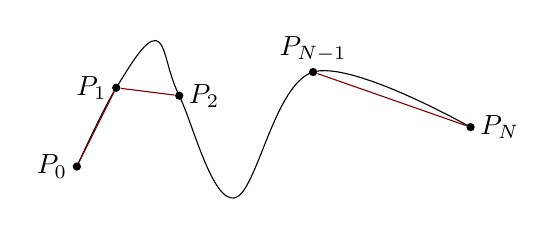
\begin{tikzpicture}
    \node [circ] (0) at (0, 0) {};
    \node [circ] (1) at (0.5, 1) {};
    \node [circ] (2) at (1.3, 0.9) {};
    \node [circ] (3) at (3, 1.2) {};
    \node [circ] (4) at (5, 0.5) {};

    \node [left] at (0) {$P_0$};
    \node [left] at (1) {$P_1$};
    \node [right] at (2) {$P_2$};
    \node [above] at (3) {$P_{N - 1}$};
    \node [right] at (4) {$P_N$};

    \draw plot [smooth, tension=0.6] coordinates {(0) (1) (1, 1.6) (2) (2, -0.4) (3) (4)};
    \draw [mred] (0) -- (1) -- (2);
    \draw [mred] (3) -- (4);
  \end{tikzpicture}
\end{center}

\begin{defi}[Length of curve]
  The length of a curve $\Gamma: [a, b] \to \R^n$ is
  \[
    \ell = \sup_{\mathcal{D}} S_{\mathcal{D}},
  \]
  if the supremum exists.
\end{defi}
Note that if $\mathcal{D}'$ is a refinement of $\mathcal{D}$ (ie. we obtain $\mathcal{D}'$ by adding more points to $\mathcal{D}$), then $S_{\mathcal{D}} \leq S_{\mathcal{D}'}$ by the triangle inequality.

We let
\[
  \mathrm{mesh}(\mathcal{D})= \max_i (t_i - t_{i - 1}).
\]
Thus if $\ell$ exists, then we have
\[
  \ell = \lim_{\mathrm{mesh}(\mathcal{D}) \to 0} s_{\mathcal{D}}.
\]
Note also that by definition,
\[
  \ell = \inf\{\tilde{\ell}: \tilde{\ell} \geq S_{\mathcal{D}}\text{ for all }\mathcal{D}\}.
\]
The definition by itself isn't too helpful, since there is no nice and easy way to check if the supremum exists. However, differentiability allows us to compute this easily:
\begin{prop}
  If $\Gamma$ is continuously differentiable (ie. $C^1$), then the length of $\Gamma$ is given by
  \[
    \length(\Gamma) = \int_a^b \|\Gamma'(t)\|\;\d t.
  \]
\end{prop}
The proof is just a careful check that the definition of the integral coincides with the definition of length.
\begin{proof}
  To simplify notation, we assume $n = 3$. However, the proof works for all possible dimensions. We write
  \[
    \Gamma(t) = (f_1(t), f_2(t), f_3(t)).
  \]
  For every $s \not= t \in [a, b]$, the mean value theorem tells us
  \[
    \frac{f_i(t) - f_i(s)}{t - s} = f'_i (\xi_i)
  \]
  for some $\xi_i \in (s, t)$, for all $i = 1, 2, 3$.

  Now note that $f_i'$ are continuous on a closed, bounded interval, and hence uniformly continuous. For all $\varepsilon \in 0$, there is some $\delta > 0$ such that $|t - s| < \delta$ implies
  \[
    |f_i'(\xi_i) - f'(\xi)| < \frac{\varepsilon}{3}
  \]
  for all $\xi \in (s, t)$. Thus, for any $\xi \in (s, t)$, we have
  \[
    \left\|\frac{\Gamma(t) - \Gamma(s)}{t - s} - \Gamma'(\xi)\right\| = \left\|\begin{pmatrix}f'_1(\xi_1)\\ f'_2(\xi_2)\\ f'_3(\xi_3)\end{pmatrix} - \begin{pmatrix}f'_1(\xi)\\ f'_2(\xi)\\ f'_3(\xi)\end{pmatrix}\right\| \leq \frac{\varepsilon}{3} + \frac{\varepsilon}{3} + \frac{\varepsilon}{3} = \varepsilon.
  \]
  In other words,
  \[
    \|\Gamma(t) - \Gamma(s) - (t - s) \Gamma'(\xi)\| \leq \varepsilon(t - s).
  \]
  We relabel $t = t_i$, $s = t_{i - 1}$ and $\xi = \frac{s + t}{2}$.
  Using the triangle inequality, we have
  \begin{multline*}
    (t_i - t_{i - 1}) \left\|\Gamma'\left(\frac{t_i + t_{i - 1}}{2}\right)\right\| - \varepsilon(t_i - t_{i - 1}) < \|\Gamma(t_i) - \Gamma(t_{i - 1}) \\
    < (t_i - t_{i - 1}) \left\|\Gamma'\left(\frac{t_i + t_{i - 1}}{2}\right)\right\| + \varepsilon(t_i - t_{i - 1}).
  \end{multline*}
  Summing over all $i$, we obtain
  \begin{multline*}
    \sum_i (t_i - t_{i - 1}) \left\|\Gamma'\left(\frac{t_i + t_{i - 1}}{2}\right)\right\| - \varepsilon(b - a) < S_{\mathcal{D}}\\
    < \sum_i (t_i - t_{i - 1}) \left\|\Gamma'\left(\frac{t_i + t_{i - 1}}{2}\right)\right\| + \varepsilon(b - a),
  \end{multline*}
  which is valid whenever $\mathrm{mesh}(\mathcal{D}) < \delta$.

  Since $\Gamma'$ is continuous, and hence integrable, we know
  \[
    \sum_i (t_i - t_{i - 1}) \left\|\Gamma'\left(\frac{t_i + t_{i - 1}}{2}\right)\right\| \to \int_a^b \|\Gamma'(t)\|\;\d t
  \]
  as $\mathrm{mesh}(\mathcal{D}) \to 0$, and
  \[
    \length(\Gamma) = \lim_{\mathrm{mesh}(\mathcal{D}) \to 0} S_\mathcal{D} = \int_a^b \|\Gamma'(t)\|\;\d t.
  \]
\end{proof}
This is all we are going to say about Euclidean space.

\section{Spherical geometry}
As the name suggests, we will be working on a two-dimensional sphere sitting in a three dimensional space.
\begin{notation}
  We write $S = S^2 \subseteq \R^3$ for the unit sphere. We write $O = \mathbf{0}$ for the origin, which is the center of the sphere.
\end{notation}

\begin{defi}[Great circle]
  A \emph{great circle} (in $S^2$) is $S^2 \cap (\text{a plane through }O)$. We also call these \emph{(spherical) lines}.
\end{defi}
We will also call these geodesics, which is a much more general term that happens to be great circles in spheres.

Given any two non-antipodal points $P, Q \in S$, there exists a unique line on $S$ through $P$ and $Q$, since there is a unique plane through $O, P, Q$ if they are not colinear.

\begin{defi}[Distance on a sphere]
  Given $P, Q \in S$, the \emph{distance} $d(P, Q)$ is the shorter of the two (spherical) line segments (ie. arcs) $PQ$ along the respective great circle. When $P$ and $Q$ are antipodal, there are infinitely many line segments between them of the same length, and the distance is $\pi$.
\end{defi}
Note that by the definition of the radian, $d(P, Q)$ is the angle between $\overrightarrow{OP}$ and $\overrightarrow{OQ}$, which is also $\cos^{-1}(\mathbf{P}\cdot \mathbf{Q})$ (where $\mathbf{P} = \overline{OP}$, $\mathbf{Q} = \overline{OQ}$).

\subsection{Triangles on a sphere}
One main object of study is spherical triangles -- they are defined just like Euclidean triangles, with $AB, AC, BC$ line segments on $S$ of length $<\pi$. The restriction of length is just merely for convenience.
\begin{center}
  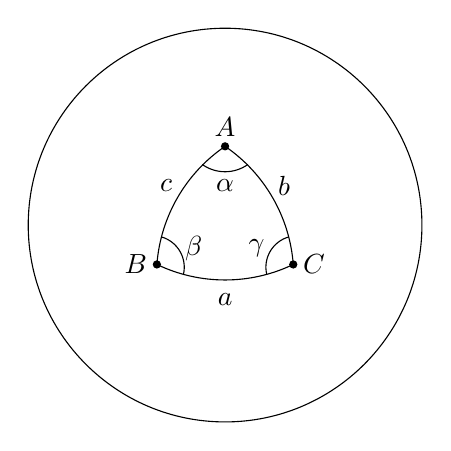
\begin{tikzpicture}
    \draw circle [radius = 2.5];
    \pgfpathmoveto{\pgfpoint{-0.86602cm}{-0.5cm}};
    \pgfpatharcto{2cm}{2cm}{0}{0}{0}{\pgfpoint{0cm}{1cm}}\pgfusepath{stroke};
    \pgfpathmoveto{\pgfpoint{0cm}{1cm}};
    \pgfpatharcto{2cm}{2cm}{0}{0}{0}{\pgfpoint{0.86602cm}{-0.5cm}}\pgfusepath{stroke};
    \pgfpathmoveto{\pgfpoint{0.86602cm}{-0.5cm}};
    \pgfpatharcto{2cm}{2cm}{0}{0}{0}{\pgfpoint{-0.86602cm}{-0.5cm}}\pgfusepath{stroke};

    \draw (0, 1) node [above] {$A$} node [circ] {};
    \draw (-0.86602, -0.5) node [left] {$B$} node [circ] {};
    \draw (0.86602, -0.5) node [right] {$C$} node [circ] {};
    \node at (-0.55, 0.5) [left] {$c$};
    \node at (0.55, 0.5) [right] {$b$};
    \node at (0, -0.75) [below] {$a$};

    \pgfpathmoveto{\pgfpoint{-0.29cm}{0.77cm}};
    \pgfpatharcto{0.5cm}{0.5cm}{0}{0}{1}{\pgfpoint{0.29cm}{0.77cm}}\pgfusepath{stroke};
    \node at (0, 0.5) {$\alpha$};

    \pgfpathmoveto{\pgfpoint{-0.81cm}{-0.15cm}};
    \pgfpatharcto{0.4cm}{0.4cm}{0}{0}{0}{\pgfpoint{-0.53cm}{-0.63cm}}\pgfusepath{stroke};
    \node at (-0.4, -0.3) {$\beta$};

    \pgfpathmoveto{\pgfpoint{0.81cm}{-0.15cm}};
    \pgfpatharcto{0.4cm}{0.4cm}{0}{0}{1}{\pgfpoint{0.53cm}{-0.63cm}}\pgfusepath{stroke};
    \node at (0.4, -0.3) {$\gamma$};
  \end{tikzpicture}
\end{center}
We will take advantage of the fact that the sphere sits in $\R^3$. We set
\begin{align*}
  \mathbf{n}_1 &= \frac{\mathbf{C}\times \mathbf{B}}{\sin a}\\
  \mathbf{n}_2 &= \frac{\mathbf{A}\times \mathbf{C}}{\sin b}\\
  \mathbf{n}_3 &= \frac{\mathbf{B}\times \mathbf{A}}{\sin c}.
\end{align*}
These are unit normals to the planes $OBC, OAC$ and $OAB$ respectively. They are pointing out of the solid $OABC$.

The angles $\alpha, \beta, \gamma$ are the angles between the planes for the respective sides. Then $0 < \alpha, \beta, \gamma < \pi$. Note that the angle between $\mathbf{n}_2$ and $\mathbf{n}_3$ is $\pi + \alpha$ (not $\alpha$ itself --- if $\alpha = 0$, then the angle between the two normals is $\pi$). So
\begin{align*}
  \mathbf{n}_2 \cdot \mathbf{n}_3 &= -\cos \alpha\\
  \mathbf{n}_3 \cdot \mathbf{n}_1 &= -\cos \beta\\
  \mathbf{n}_1 \cdot \mathbf{n}_2 &= -\cos \gamma.
\end{align*}
We have the following theorem:
\begin{thm}[Spherical cosine rule]
  \[
    \sin a \sin b \cos \gamma = \cos c - \cos a \cos b.
  \]
\end{thm}

\begin{proof}
  We use the fact from IA Vectors and Matrices that
  \[
    (\mathbf{C}\times \mathbf{B}) \cdot (\mathbf{A} \times \mathbf{C}) = (\mathbf{A}\cdot \mathbf{C})(\mathbf{B}\cdot \mathbf{C}) - (\mathbf{C} \cdot \mathbf{C})(\mathbf{B}\cdot \mathbf{A}).
  \]
  This follows from the double-epsilon identity
  \[
    \varepsilon_{ijk}\varepsilon_{imn} = \delta_{jm}\delta_{kn} - \delta_{jn}\delta_{km}.
  \]
  In our case, since $\mathbf{C}\cdot \mathbf{C} = 1$, the right hand side is
  \[
    (\mathbf{A}\cdot \mathbf{C}) (\mathbf{B}\cdot \mathbf{C}) - (\mathbf{B}\cdot \mathbf{A}).
  \]
  Thus we have
  \begin{align*}
    -\cos \gamma &= \mathbf{n}_1 \cdot \mathbf{n}_2\\
    &= \frac{\mathbf{C}\times \mathbf{B}}{\sin a} \cdot \frac{\mathbf{A}\times \mathbf{C}}{\sin b} = \frac{(\mathbf{A}\cdot \mathbf{C})(\mathbf{B}\cdot \mathbf{C}) - (\mathbf{B}\cdot \mathbf{A})}{\sin a \sin b}\\
    &= \frac{\cos b\cos a - \cos c}{\sin a \sin b}.
  \end{align*}
\end{proof}

\begin{cor}[Pythagoras theorem]
  If $\gamma = \frac{\pi}{2}$, then
  \[
    \cos c = \cos a \cos b.
  \]
\end{cor}

Analogously, we have a spherical sine rule.
\begin{thm}[Spherical sine rule]
  \[
    \frac{\sin a}{\sin \alpha} = \frac{\sin b}{\sin \beta} = \frac{\sin c}{\sin \gamma}.
  \]
\end{thm}

\begin{proof}
  We use the fact that
  \[
    (\mathbf{A}\times \mathbf{C}) \times (\mathbf{C}\times \mathbf{B}) = (\mathbf{C}\cdot (\mathbf{B}\times \mathbf{A}))\mathbf{C},
  \]
  which we again are not bothered to prove again. The left hand side is
  \[
    -(\mathbf{n}_1 \times \mathbf{n}_2) \sin a \sin b
  \]
  Since the angle between $\mathbf{n}_1$ and $\mathbf{n}_2$ is $\pi + \gamma$, we know $\mathbf{n}_1 \times \mathbf{n}_2 = \mathbf{C}\sin \gamma$. Thus the left hand side is
  \[
    -\mathbf{C} \sin a \sin b \sin \gamma.
  \]
  Thus we know
  \[
    \mathbf{C}\cdot (\mathbf{A} \times \mathbf{B}) = \sin a\sin b \sin \gamma.
  \]
  However, since the scalar triple product is cyclic, we know
  \[
    \mathbf{C}\cdot (\mathbf{A}\times \mathbf{B}) = \mathbf{A}\cdot (\mathbf{B} \times \mathbf{C}).
  \]
  In other words, we have
  \[
    \sin a \sin b \sin \gamma = \sin b \sin c \sin \alpha.
  \]
  Thus we have
  \[
    \frac{\sin \gamma}{\sin c} = \frac{\sin \alpha}{\sin a}.
  \]
  Similarly, we know this is equal to $\frac{\sin \beta}{\sin b}$.
\end{proof}

Recall that for small $a, b, c$, we know
\[
  \sin a = a + O(a^3).
\]
Similarly,
\[
  \cos a = 1 - \frac{a^2}{2} + O(a^4).
\]
As we take the limit $a, b, c \to 0$, the spherical sine and cosine rules become the usual Euclidean versions. For example, the cosine rule becomes
\[
  ab \cos \gamma = 1 - \frac{c^2}{2} - \left(1 - \frac{a^2}{2}\right)\left(1 - \frac{b^2}{2}\right) + O(\|(a, b, c)\|^3).
\]
Rearranging gives
\[
  c^2 = a^2 + b^2 - 2ab \cos \gamma + O(\|(a, b, c,)\|^3).
\]
The sine rule transforms similarly as well. This is what we would expect, since making $a, b, c$ small is equivalent to zooming into the surface of the sphere, and it looks more and more like flat space.

Note that if $\gamma = \pi$, it then follows that $C$ is in the line segment given by $AB$. So $c = a + b$. Otherwise, we get
\[
  \cos c > \cos a \cos b - \sin a \sin b = \cos(a + b),
\]
since $\cos \gamma < 1$. Since $\cos$ is decreasing on $[0, \pi]$, we know
\[
  c < a + b.
\]
\begin{cor}[Triangle inequality]
  For any $P, Q, R \in S^2$, we have
  \[
    d(P, Q) + d(Q, R) \geq d(P, R),
  \]
  with equality if and only if $Q$ lies is in the line segment $PR$ of shortest length.
\end{cor}

\begin{proof}
  The only case left to check is if $d(P, R) = \pi$. But then they are antipodal points, and $Q$ lies in the line through $PR$. So equality holds.
\end{proof}
Thus, we find that $(S^2, d)$ is a metric space.

We now prove a statement that sounds really obvious:
\begin{prop}
  Given a curve $\Gamma$ on $S^2 \subseteq \R^3$ from $P$ to $Q$, we have $\ell = \length(\Gamma) \geq d(P, Q)$. Moreover, if $\ell = d(P, Q)$, then the image of $\Gamma$ is a spherical line segment $PQ$.
\end{prop}

\begin{proof}
  Let $\Gamma: [0, 1] \to S$ and $\ell = \length(\Gamma)$. Then for any dissection $\mathcal{D}$ of $[0, 1]$, say $0 = t_0 < \cdots < t_N = 1$, write $P_i = \Gamma(t_i)$. We define
  \[
    \tilde{S}_{\mathcal{D}} = \sum_i d(P_{i - 1}, P_i) > S_{\mathcal{D}} = \sum_i |\overrightarrow{P_{i - 1}P_i}|,
  \]
  where the length in the right hand expression is the distance in Euclidean $3$-space.

  Now suppose $\ell < d(P, Q)$. Then there is some $\varepsilon > 0$ such that $\ell(1 + \varepsilon) < d(P, Q)$.

  Recall from basic trigonometric that if $\theta > 0$, then $\sin \theta < \theta$. Also,
  \[
    \frac{\sin \theta}{\theta} \to 1\text{ as }\theta \to 0.
  \]
  Thus we have
  \[
    \theta \leq (1 + \varepsilon) \sin \theta.
  \]
  for small $\theta$. What we really want is the double of this:
  \[
    2\theta \leq (1 + \varepsilon) 2\sin \theta.
  \]
  This is useful since these lengths appear in the following diagram:
  \begin{center}
    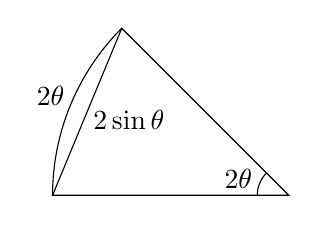
\begin{tikzpicture}
      \draw (-3, 0) -- (0, 0) -- (-2.121, 2.121) -- cycle node [pos=0.55, right] {$2 \sin \theta$};
      \draw (-3, 0) arc (180:135:3) node [pos=0.55, left] {$2 \theta$};

      \draw (-0.4, 0) arc(180:135:0.4) node [pos=0.7, left] {$2\theta$};
    \end{tikzpicture}
  \end{center}
  This means for $P, Q$ sufficiently close, we have $d(P, Q) \leq (1 + \varepsilon) |\overrightarrow{PQ}|$.

  From Analysis II, we know $\Gamma$ is uniformly continuous on $[0, 1]$. So we can choose $\mathcal{D}$ such that
  \[
    d(P_{i - 1}, P_i) \leq (1 + \varepsilon)|\overrightarrow{P_{i - 1}P_i}|
  \]
  for all $i$. So we know that for sufficiently fine $\mathcal{D}$,
  \[
    \tilde{S}_{\mathcal{D}} \leq (1 + \varepsilon) S_\mathcal{D} < d(P, Q),
  \]
  since $S_\mathcal{D} \to \ell$. However, by the triangle inequality $\tilde{S}_\mathcal{D} \geq d(P, Q)$. This is a contradiction. Hence we must have $\ell \geq d(P, Q)$.

  Suppose now $\ell = d(P, Q)$ for some $\Gamma: [0, 1] \to S$, $\ell = \length(\Gamma)$. Then for every $t \in [0, 1]$, we have
  \begin{align*}
    d(P, Q) = \ell &= \length \Gamma|_{[0, t]} + \length \Gamma|_{[t, 1]} \\
    &\geq d(P, \Gamma(t)) + d(\Gamma(t), Q)\\
    &\geq d(P, Q).
  \end{align*}
  Hence we must have equality all along the way, ie.
  \[
    d(P, Q) = d(P, \Gamma(t)) + d(\Gamma(t), Q)
  \]
  for all $\Gamma(t)$.

  However, this is possible only if $\Gamma(t)$ lies on the shorter spherical line segment $PQ$, as we have previously proved. So done.
\end{proof}

Note that if $\Gamma$ is a curve of minimal length from $P$ to $Q$, then $\Gamma$ is a spherical line segment. Further, from the proof of this proposition, we know $\length \Gamma|_{[0, t]} = d(P, \Gamma(t))$ for all $t$. So the parametrisation of $\Gamma$ is monotonic. Such a $\Gamma$ is called a \emph{minimizing geodesic}.

On example sheet 1, question 4, you will be asked to do the Euclidean version of the above.

We are now going to prove a theorem about the area of spherical triangles. This is in fact a special case of the Gauss-Bonnet theorem. We will only state and prove the special case here, and leave the general case for a later time.

\begin{prop}[Gauss-Bonnet theorem for $S^2$]
  If $\Delta$ is a spherical triangle with angles $\alpha, \beta, \gamma$, then
  \[
    \area (\Delta) = (\alpha + \beta + \gamma) - \pi.
  \]
\end{prop}

\newcommand\filllune[9]{
  \pgfmathsetmacro{\xx}{#3 * cos(#4)};
  \pgfmathsetmacro{\xy}{#3 * sin(#4)};
  \pgfmathsetmacro{\yx}{#3 * cos(#5)};
  \pgfmathsetmacro{\yy}{#3 * sin(#5)};

  \color{#8};
  \pgfsetfillopacity{0.6};
  \pgfpathmoveto{\pgfpoint{#1}{#2}};
  \pgfpatharcto{#3 cm}{#6 cm}{#4}{0}{1}{\pgfpoint{-\xx cm}{-\xy cm}};
  \pgfpatharcto{#3 cm}{#3 cm}{0}{0}{#9}{\pgfpoint{-\yx cm}{-\yy cm}};
  \pgfpatharcto{#3 cm}{#7 cm}{#5}{0}{int(1-#9)}{\pgfpoint{#1}{#2}};
  \pgfusepath{fill};

  \pgfpathmoveto{\pgfpoint{#1}{#2}};
  \pgfpatharcto{#3 cm}{#6 cm}{#4}{0}{0}{\pgfpoint{\xx cm}{\xy cm}};
  \pgfpatharcto{#3 cm}{#3 cm}{0}{0}{#9}{\pgfpoint{\yx cm}{\yy cm}};
  \pgfpatharcto{#3 cm}{#7 cm}{#5}{0}{#9}{\pgfpoint{#1}{#2}};
  \pgfusepath{fill};

  \pgfsetfillopacity{0.11};
  \pgfpathmoveto{\pgfpoint{-#1}{-#2}};
  \pgfpatharcto{#3 cm}{#6 cm}{#4}{0}{0}{\pgfpoint{-\xx cm}{-\xy cm}};
  \pgfpatharcto{#3 cm}{#3 cm}{0}{0}{#9}{\pgfpoint{-\yx cm}{-\yy cm}};
  \pgfpatharcto{#3 cm}{#7 cm}{#5}{0}{#9}{\pgfpoint{-#1}{-#2}};
  \pgfusepath{fill};

  \pgfpathmoveto{\pgfpoint{-#1}{-#2}};
  \pgfpatharcto{#3 cm}{#6 cm}{#4}{0}{1}{\pgfpoint{\xx cm}{\xy cm}};
  \pgfpatharcto{#3 cm}{#3 cm}{0}{0}{#9}{\pgfpoint{\yx cm}{\yy cm}};
  \pgfpatharcto{#3 cm}{#7 cm}{#5}{0}{int(1-#9)}{\pgfpoint{-#1}{-#2}};
  \pgfusepath{fill};
}

\begin{proof}
  We start with the concept of a double lune. A \emph{double lune} with angle $0 < \alpha < \pi$ is two regions $S$ cut out by two planes through a pair of antipodal points, where $\alpha$ is the angle between the two planes.
  \begin{center}
    \begin{tikzpicture}
      \pgfdeclarelayer{col}
      \pgfsetlayers{col,main}
      \pgfmathsetmacro{\radius}{2.5}
      \pgfmathsetmacro{\ct}{20}
      \pgfmathsetmacro{\crad}{1.3}
      \pgfmathsetmacro{\dt}{70}
      \pgfmathsetmacro{\drad}{0.5}

      \draw circle [radius = \radius];

      \draw [name path=c1, rotate=\ct] (\radius, 0) arc(0:180:{\radius} and {\crad});
      \draw [opacity=0.6, name path=d1, rotate=\ct, dashed] (\radius, 0) arc(0:-180:{\radius} and {\crad});

      \draw [name path=c2, rotate=\dt] (\radius, 0) arc(0:180:{\radius} and {\drad});
      \draw [opacity=0.6, name path=d2, rotate=\dt, dashed] (\radius, 0) arc(0:-180:{\radius} and {\drad});

      \path [name intersections={of=c1 and c2,by=A}];
      \path [name intersections={of=d1 and d2,by=A'}];
      \node [circ] at (A) {};
      \node [circ] at (A') {};

      \node [anchor = south east] at (A) {$A$};
      \node [anchor = south east] at (A') {$A'$};

      \getCoord{\ax}{\ay}{A};
      \getCoord{\aax}{\aay}{A'};
      \begin{pgfonlayer}{col}
        \filllune{\ax}{\ay}{\radius}{\ct}{\dt}{\crad}{\drad}{mblue}{1};
      \end{pgfonlayer}

    \end{tikzpicture}
  \end{center}
  It is not hard to show that the area of a double lune is $4 \alpha$, since the area of the sphere is $4\pi$.

  Now note that our triangle $\Delta = ABC$ is the intersection of 3 \emph{single} lunes, with each of $A, B, C$ as the pole (in fact we only need two, but it is more convenient to talk about $3$).
  \begin{center}
    \begin{tikzpicture}
      \pgfdeclarelayer{col}
      \pgfsetlayers{col,main}
      \pgfmathsetmacro{\radius}{2.5}
      \pgfmathsetmacro{\ct}{20}
      \pgfmathsetmacro{\crad}{1.3}
      \pgfmathsetmacro{\dt}{70}
      \pgfmathsetmacro{\drad}{0.5}
      \pgfmathsetmacro{\et}{140}
      \pgfmathsetmacro{\erad}{0.5}

      \draw circle [radius = \radius];

      \draw [name path=c1, rotate=\ct] (\radius, 0) arc(0:180:{\radius} and {\crad});
      \draw [opacity=0.6, name path=c2, rotate=\ct, dashed] (\radius, 0) arc(0:-180:{\radius} and {\crad});

      \draw [name path=d1, rotate=\dt] (\radius, 0) arc(0:180:{\radius} and {\drad});
      \draw [opacity=0.6, name path=d2, rotate=\dt, dashed] (\radius, 0) arc(0:-180:{\radius} and {\drad});

      \draw [name path=e1, rotate=\et] (\radius, 0) arc(0:180:{\radius} and {\erad});
      \draw [opacity=0.6, name path=e2, rotate=\et, dashed] (\radius, 0) arc(0:-180:{\radius} and {\erad});

      \path [name intersections={of=c1 and d1,by=A}];
      \path [name intersections={of=c2 and d2,by=A'}];
      \node [circ] at (A) {};
      \node [opacity=0.6, circ] at (A') {};
      \node [anchor = south east] at (A) {$A$};
      \node [opacity=0.6, anchor = south east] at (A') {$A'$};

      \path [name intersections={of=c1 and e1,by=B}];
      \path [name intersections={of=c2 and e2,by=B'}];
      \node [circ] at (B) {};
      \node [opacity=0.6, circ] at (B') {};
      \node [left] at (B) {$B$};
      \node [opacity=0.6, right] at (B') {$B'$};

      \path [name intersections={of=d1 and e1,by=C}];
      \path [name intersections={of=d2 and e2,by=C'}];
      \node [circ] at (C) {};
      \node [opacity=0.6, circ] at (C') {};
      \node [right] at (C) {$C$};
      \node [opacity=0.6, right] at (C') {$C'$};

      \getCoord{\ax}{\ay}{A};
      \getCoord{\bx}{\by}{B};
      \getCoord{\cx}{\cy}{C};

      \begin{pgfonlayer}{col}
        \filllune{\ax}{\ay}{\radius}{\ct}{\dt}{\crad}{\drad}{mblue}{1};
        \filllune{\bx}{\by}{\radius}{\ct}{180+\et}{\crad}{\erad}{mgreen}{0};
        \filllune{\cx}{\cy}{\radius}{\dt}{\et}{\drad}{\erad}{morange}{1};
      \end{pgfonlayer}
    \end{tikzpicture}
  \end{center}
  Therefore $\Delta$ together with its antipodal partner $\Delta'$ is a subset of each of the 3 double lunes with areas $4\alpha, 4\beta, 4\gamma$. Also, the union of all the double lunes cover the whole sphere, and overlap at exactly $\Delta$ and $\Delta'$.
  Thus
  \[
    4(\alpha + \beta + \gamma) = 4\pi + 2(\area(\Delta) + \area(\Delta')) = 4\pi + 4 \area(\Delta).
  \]
\end{proof}
Note that unlike on Euclidean space, we have $\alpha + \beta + \gamma > \pi$. As we take the limit $\area(\Delta) \to 0$, we get $\alpha + \beta + \gamma \to \pi$, as expected, since the space looks more and more like Euclidean space as we zoom in.

Moreover, if $M$ is a convex $n$-gon on $S^2$ (with $n \geq 3$), ie. if $P, Q \in M$, then the shorter line segment $PQ$ lies in $M$, and the interior angles are $\alpha_1, \cdots, \alpha_n$, then
\[
  \area(M) = \sum_1^n \alpha_i - (n - 2) \pi.
\]
This is easy to show by cutting the polygon up into triangles.

\subsubsection*{M\"obius geometry}
One other useful thing in the study of spherical geometry is M\"obius transformations.

Consider $\C_\infty = \C \cup \{\infty\}$, the extended complex plane, with coordinates $\zeta \in \C_\infty$. One useful notion is the \emph{stereographic projection} $\pi: S^2 \to \C_\infty$, which is a bijection given by
\begin{center}
  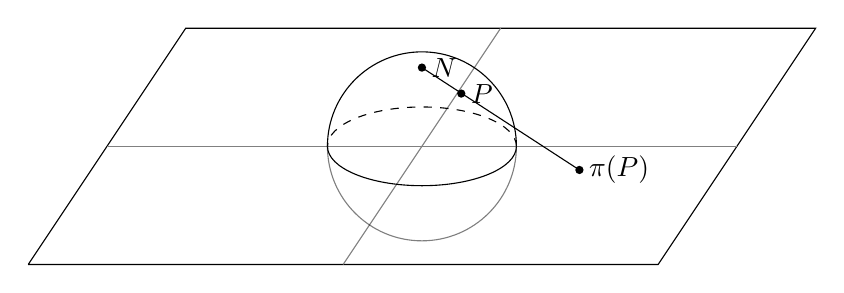
\begin{tikzpicture}
    \draw (0, 0) -- (8, 0) -- (10, 3) -- (2, 3) -- (0, 0);
    \draw [gray] (1, 1.5) -- (9, 1.5);
    \draw [gray] (4, 0) -- (6, 3);
    \draw (6.2, 1.5) arc(0:180:1.2);
    \draw [opacity=0.5] (6.2, 1.5) arc(0:-180:1.2);
    \draw (6.2, 1.5) arc(0:-180:1.2 and 0.5);
    \draw [dashed] (6.2, 1.5) arc(0:180:1.2 and 0.5);

    \node [circ] at (5, 2.5) {};
    \node at (5, 2.5) [right] {$N$};

    \node [circ] at (5.5, 2.17) {};
    \node at (5.5, 2.17) [right] {$P$};

    \draw (5, 2.5) -- (7, 1.2) node [circ] {} node [right] {$\pi(P)$};
  \end{tikzpicture}
\end{center}
\[
  \pi(P) = (\text{line } PQ)\cap \{z = 0\},
\]
which is well defined except where $P = N$, in which case we define $\pi(N) = \infty$.

To give an explicit formula for this, consider the cross-section through the plane $ONP$.
\begin{center}
  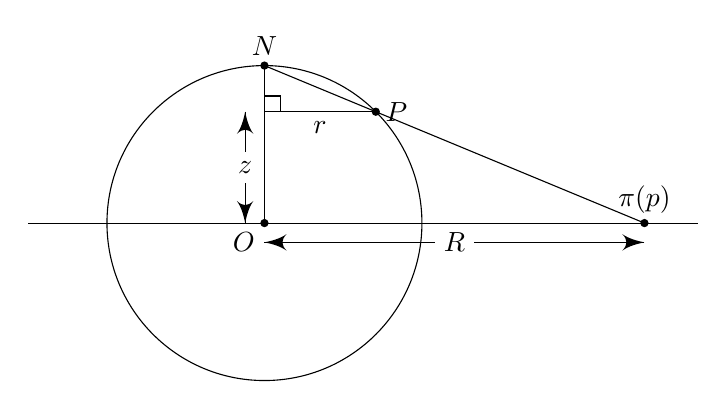
\begin{tikzpicture}
    \node [circ] {};
    \node [anchor = north east] {$O$};
    \draw circle [radius=2];
    \draw (-3, 0) -- (5.5, 0);
    \draw (0, 0) -- (0, 2) node [circ] {} node [above] {$N$};
    \draw (0, 1.414) -- (1.414, 1.414) node [pos=0.5, below] {$r$} node [right] {$P$} node [circ] {};
    \draw (0.2, 1.414) -- +(0, 0.2) -- +(-0.2, 0.2);

    \draw [<->] (-0.245, 0) -- +(0, 1.414) node [fill=white, pos=0.5] {$z$};
    \draw (0, 2) -- (4.8259, 0) node [circ] {} node [above] {$\pi(p)$};

    \draw [<->] (0, -0.245) -- +(4.8259, 0) node [fill=white, pos=0.5] {$R$};
  \end{tikzpicture}
\end{center}
We notice similar triangles
\[
  \frac{r}{R} = \frac{1 - z}{1}.
\]
Then we obtain the formula
\[
  \pi(x, y, z) = \frac{x + iy}{1 - z}
\]
\begin{lemma}
  if $\pi': S^2 \to C_{\infty}$ denotes the stereographic projection from the South Pole instead, then
  \[
    \pi'(P) = \frac{1}{\overline{\pi(P)}}.
  \]
\end{lemma}

\begin{proof}
  Let $P(x, y, z)$. Then
  \[
    \pi(x, y, z) = \frac{x + iy}{1 - z}.
  \]
  Then we have
  \[
    \pi'(x, y, z) = \frac{x + iy}{1 + z},
  \]
  since we have just flipped the $z$ axis around. So we have
  \[
    \overline{\pi(P)}\pi'(P) = \frac{x^2 + y^2}{1 - z^2} =1,
  \]
  noting that we have $x^2 + y^2 + z^2 = 1$ since we are on the unit sphere.
\end{proof}

We can use this to infer that $\pi' \circ \pi^{-1}: C_{\infty} \to C_{\infty}$ takes $\zeta \mapsto \frac{1}{\bar{\zeta}}$, which is the inversion in the unit circle $|\zeta| = 1$.
\end{document}
